\section{\acs{RS} Scheme Simulation}
\label{sec:fec_scheme_simulation}

To be able to investigate the effect that different \ac{RS} coding strengths have on decoded \ac{PRR}, we needed a way to compare experiment results.
Due to the difficulty of recreating the \emph{exact} same conditions for several series of real world experiments, we chose to create and use a trace-based simulator to apply the bit error patterns of an original experiment onto several new $RS(n, k)$ encoded random payloads.

By interpreting the $RS(80, 70)$ encoded random payload as pseudo-random in the context of Section~\ref{sec:packet_reception_rate}, we made dual-use of that experiment.
This allows us an in-depth description of the link conditions onto which we built our analysis of \ac{RS} performance.

We will next describe how we use the raw data of this experiment as an input for our simulation, by extracting its \ac{BER} patterns and applying them onto new payload, and discuss accuracy and limitations.

\subsection{Design}

The simulator re-runs an original experiment message-by-message over its log, and outputs a new one.
We only simulate \ac{BER} patterns, all other properties of the link, such as link qualifiers, temperature, transmission power, are copied from the original link, as visualized in Figure~\ref{fig:simulator_design}.
In addition, if a message was not received by a receiver, we simply preserve it as a timeout, to make later comparison of the simulated results with the real experiments much easier.

Our simulator also works with experiments where a transmitted message is received by multiple receivers as in Section~\ref{subsec:effects_of_board_layout}.
In such a case, the simulator will apply its algorithm to every received message.

\begin{figure}[t]
	\centering
	\tikzset{
	    %Define standard arrow tip
	    >=stealth',
	    %Define style for boxes
	    punkt/.style={
	           rectangle,
	           rounded corners,
	           draw=black, very thick,
	           text width=2cm,
	           minimum height=1cm,
	           text centered},
	    % Define arrow style
	    pil/.style={
	           ->,
	           very thick,
	           shorten <=2pt,
	           shorten >=2pt,}
	}
	\begin{tikzpicture}

		\fill[color=slightgray, rounded corners] (1.4,-4) rectangle (11,-2);

		\node[punkt] (input) {Input Message(s)};
 		\node[punkt, right=0.8cm of input] (parser) {Parser};
 		\node[punkt, right=3.85cm of parser] (formatter) {Formatter};
 		\node[punkt, right=0.8cm of formatter] (output) {Output Message};

 		\node[punkt, below=2cm of parser, fill=white] (analyzer) {Analyzer};
 		\node[punkt, below=2cm of formatter, fill=white] (corruptor) {Corrupter};
 		\node[right=0.85cm of corruptor] (payload) {New Payload};

 		\draw[pil] (input) -- (parser);
 		\draw[pil] (parser) -- (formatter) node[midway, below] {LQI, RSSI};
 		\path (parser) -- (formatter) node[midway, above] {Temperature};
 		\draw[pil] (formatter) -- (output);

 		\draw[pil] (parser) -- (analyzer) node[midway, left] {Original Payload(s)};
 		\draw[pil] (analyzer) -- (corruptor) node[midway, above] {BER pattern};
 		\draw[pil] (payload) -- (corruptor);
 		\draw[pil] (corruptor) -- (formatter) node[midway, right] {New Corrupted Payload};

 		\draw[pil] (input) edge[bend left=25] node[below]{Timeout} (output);

		% \draw (-1.2,-5) rectangle (13.8,1);
	\end{tikzpicture}
	\caption{Schematic design of our trace-based simulator: the payloads of multiple original messages can be analyzed to extract the \ac{BER} pattern, which is then applied to new payload.}
	\label{fig:simulator_design}
\end{figure}


\paragraph{Pattern Extraction}

Since we know that the \ac{BER} pattern is different for every of the 16 4-bit symbols, we need to generate a corruption probability for each bit within every symbol.
For that we sum up the bit errors per bit \emph{per symbol} for every original received message in the experiment in a corruption table.
The corruption table is then normalized for the occurrence of the respective symbol in the original message to yield a relative bit error occurrences \emph{per symbol} for this specific link.

This table can be averaged over several links using a sliding window, which reduces noise and increases the likelihood of seeing all symbols with their respective bit error patterns at least once.
This will create a corruption table of \emph{average} bit error probabilities per symbol over one or more messages.
We also average the distribution of bit error burst lengths over these messages in a burst error table.
Both the corruption and the burst error table will then be handed over to the corruption generator.

Since these tables are generated on-the-fly entirely from an experiment log, even the anomalous patterns described in Section~\ref{subsec:pattern_anomalies} can be extracted.

\paragraph{Pattern Application}

A corruption pattern is generated by randomly corrupting each new symbol with the probability defined in the bit error table.
This corruption pattern needs to be adapted for the burst error distribution of the original message by lengthening single bit errors accordingly.

The corruption sequence is applied to the new payload defined by us and written out as a new received message of the original link.

\paragraph{Limitations}

Since we map and apply bit error distribution \emph{per symbol}, every symbol must be available in the original payload at least once for this table to be complete.
Experiment logs with constant payload in which not every symbol is available should be avoided.
For random payload our message size of 93 bytes yields 186 symbols, for which it is unlikely to not see every 16 symbols at least once.

Another limitation is our modeling of the burst error distribution.
By ``simply'' applying the collected bit error table by symbol onto new payload, we are effectively interleaving the original burst errors and therefore obscuring this property of the original link.
With our simple simulation, we can only add burst errors to correct for relative occurrence compared to the original frame, but not willfully ``place'' these burst errors at the correct position to achieve the distinct burst error properties of the original link.

\subsection{Accuracy}
\label{subsec:simulation_accuracy}

To evaluate the performance of the simulator, we ran it on experiment traces containing constant payloads as well as $RS(80,70)$ encoded payloads.
By tuning the link input window size and the burst error generator, we were able to replicate similar enough bit error patterns for our purposes.
We found best accuracy with a window size of two messages.

\paragraph{Bit Error Distribution Patterns}

Figure~\ref{fig:8mote_xl_xor_simulation} and \ref{fig:8mote_s_simulation} show the bit error pattern resulting of simulating XL and S magnitudes of the experiment described in Subsection~\ref{subsec:effects_of_board_layout}.
Compared to the original patterns in Figure~\ref{fig:8mote_bit_errors}, the simulation generates a less noisy footprint with less amplitude, which makes the differences in symbols clearly visible.
This is, of course, due to the averaging during the symbol error construction that is accompanied with the smoothing of these values.

\paragraph{Burst Error Distribution}

The limitations of our burst error modeling clearly show in the burst error graph in Figure~\ref{fig:8mote_xl_burst_simulation} of the simulation. In comparison to Figure~\ref{fig:8mote_burst_error}, the simulated corruption does not exhibit the drop between 4/5-bit and 8/9-bit bursts and generates longer bursts more frequently.

\begin{figure}[t]
	\subfigure[Simulated XL bit error pattern.] {
		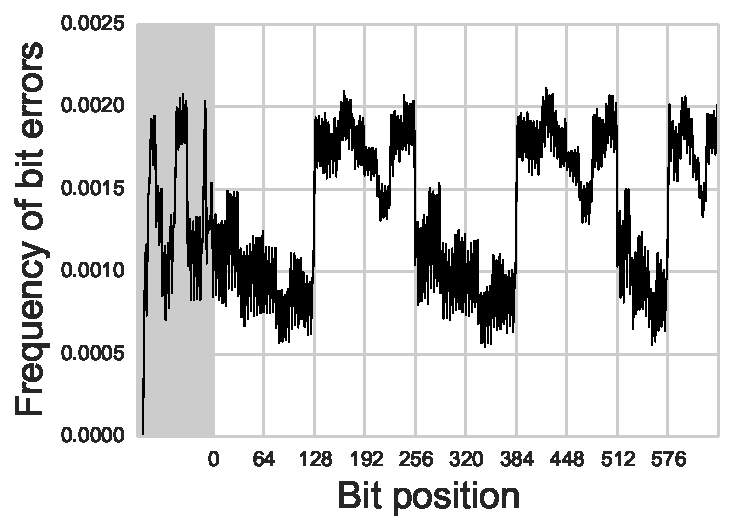
\includegraphics[width=0.475\columnwidth]{figures/8mote_0-5_xor_simulation}
		\label{fig:8mote_xl_xor_simulation}
	}
	\subfigure[Simulated S bit error pattern.] {
		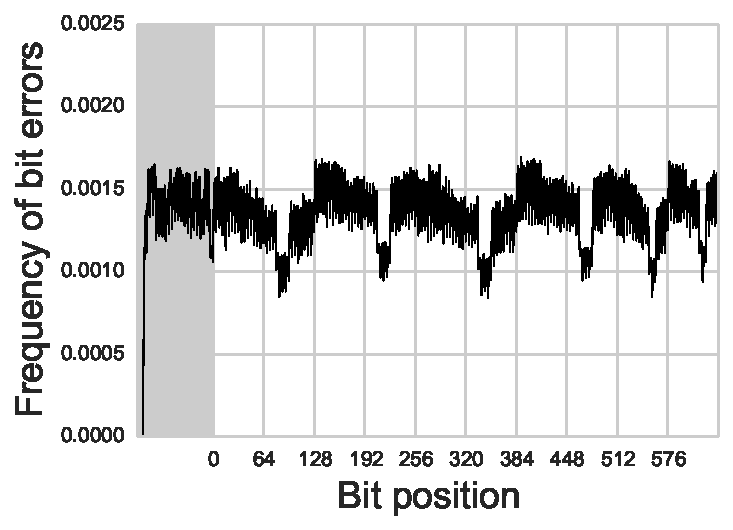
\includegraphics[width=0.475\columnwidth]{figures/8mote_2-7_xor_simulation}
		\label{fig:8mote_s_simulation}
	}
	\subfigure[Simulated XL burst error length.] {
		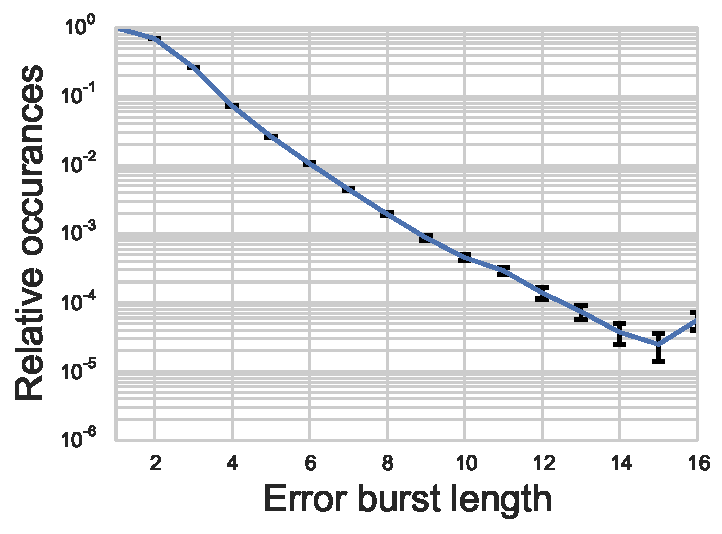
\includegraphics[width=0.475\columnwidth]{figures/8mote_0-5_burst_simulation}
		\label{fig:8mote_xl_burst_simulation}
	}
	\subfigure[Simulated S burst error length.] {
		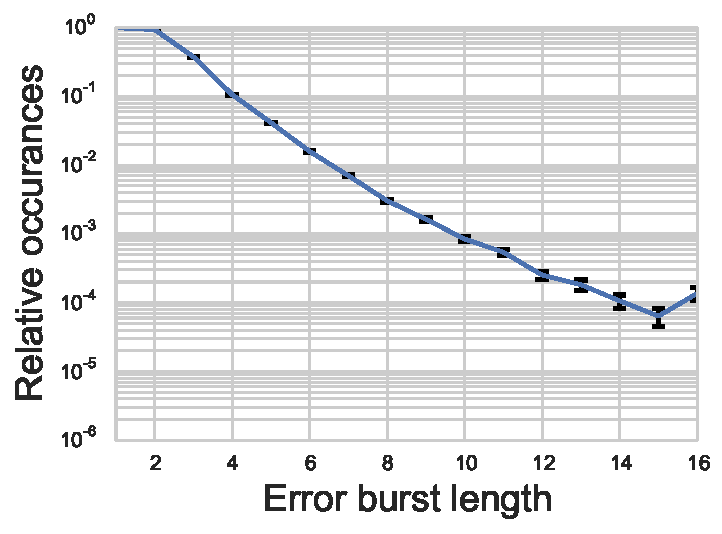
\includegraphics[width=0.475\columnwidth]{figures/8mote_2-7_burst_simulation}
		\label{fig:8mote_s_burst_simulation}
	}
	\caption{Error patterns of simulated constant payload using traces with constant payload. The error bars denote 99\% confidence intervals.}
	\label{fig:8mote_bit_errors_simulation}
\end{figure}

\paragraph{Packet Reception Rate}

To compare the overall number of corrupted messages of the original with the simulated link, we plotted the normalized \ac{PRR} of our original experiment with $RS(80,70)$ encoded payload and the simulation of that experiment with the same payload, as shown in Figures~\ref{fig:prr_link_01_fec} and \ref{fig:prr_link_10_fec} respectively.
To be able to compare the \ac{PRR} of encoded and non-encoded payload, we only evaluate the first $k=70$ bytes in the payload.
The timeouts shown in gray are the same for the simulation, since they are copied from the original, as mentioned before.

While the total amount of corrupted messages in the simulated link is the same as in the original link, as exemplified by the very similar error-free reception curves in the plots, error-free \ac{RS} decoded receptions yields slightly worse results, especially in areas with high byte error count, as visible in Figure~\ref{fig:prr_link_01_receiver_fec} and \ref{fig:prr_link_10_transmitter_fec}.
This shows that in these areas, the simulator overshoots the target bit error distribution of the original messages, and therefore undershoots the \ac{RS} decoded \ac{PRR} of the original link.
In the worst case, the simulated \ac{RS} performance is underestimated compared to reality, which is sufficient for our assessments.

\begin{figure}[t]
	\subfigure[Comparison of link~\ref{fig:prr_link_01_transmitter}.] {
		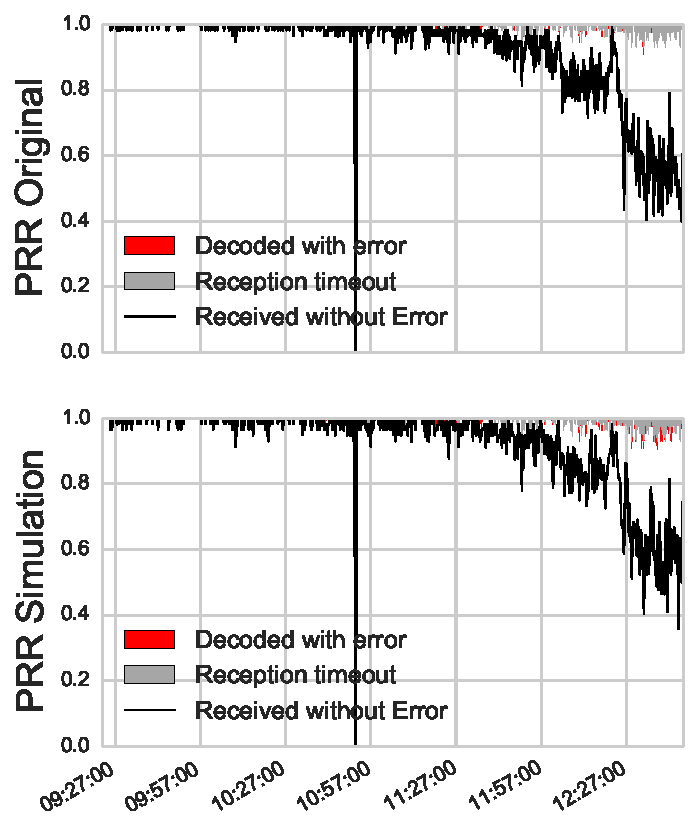
\includegraphics[width=0.475\columnwidth]{figures/fec_scheme_box0_box1_os_0-1_Throughput}
		\label{fig:prr_link_01_transmitter_fec}
	}
	\subfigure[Comparison of link~\ref{fig:prr_link_01_receiver}.] {
		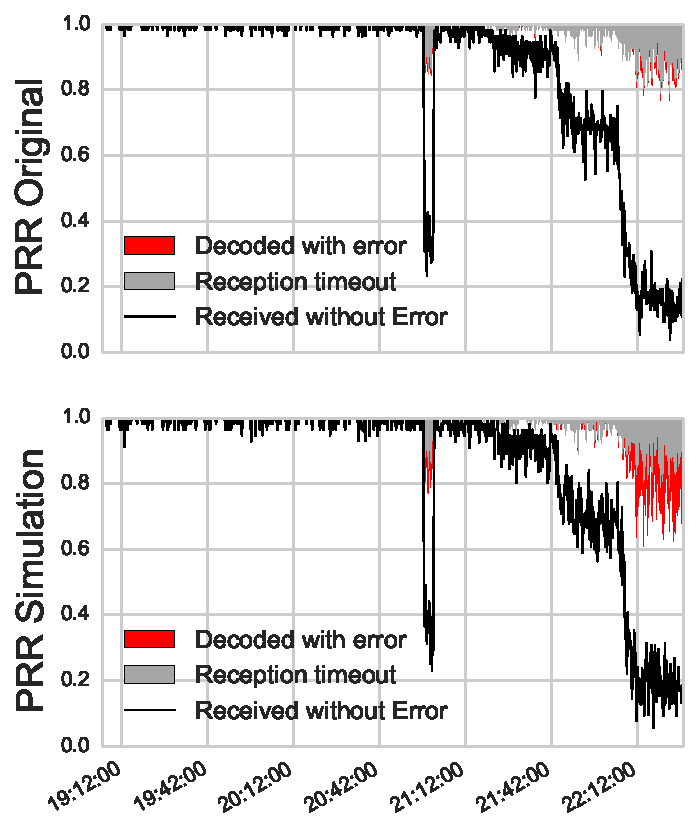
\includegraphics[width=0.475\columnwidth]{figures/fec_scheme_box1_box0_os_0-1_Throughput}
		\label{fig:prr_link_01_receiver_fec}
	}
	\caption{Original and simulated \acs{PRR} of the two $RS(80,70)$ encoded links of Figure~\ref{fig:prr_link_01}. Note the drop in simulated \acs{RS} decoded \acs{PRR} in (b).}
	\label{fig:prr_link_01_fec}
\end{figure}

\begin{figure}[t]
	\subfigure[Comparison of link~\ref{fig:prr_link_10_receiver}.] {
		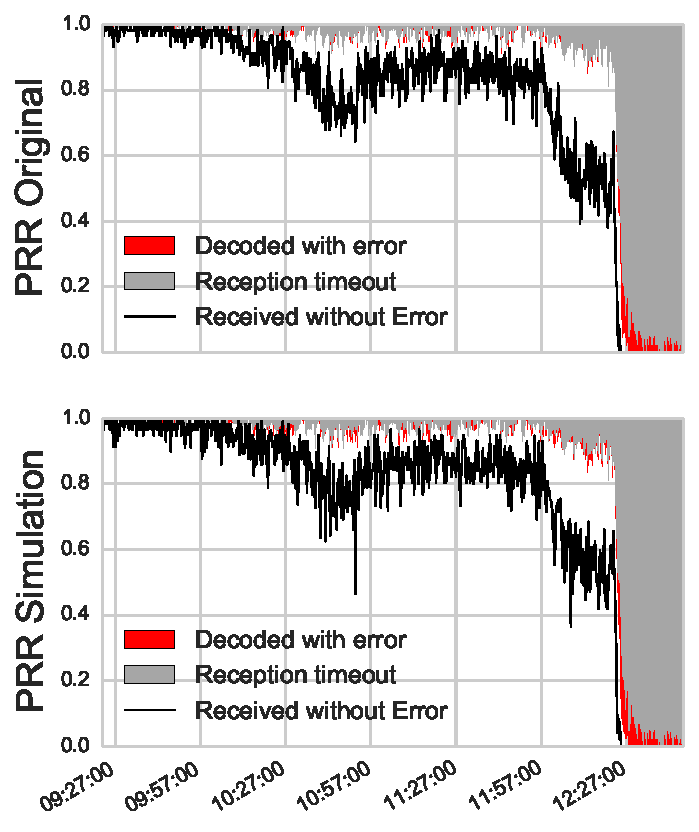
\includegraphics[width=0.475\columnwidth]{figures/fec_scheme_box0_box1_os_1-0_Throughput}
		\label{fig:prr_link_10_receiver_fec}
	}
	\subfigure[Comparison of link~\ref{fig:prr_link_10_transmitter}.] {
		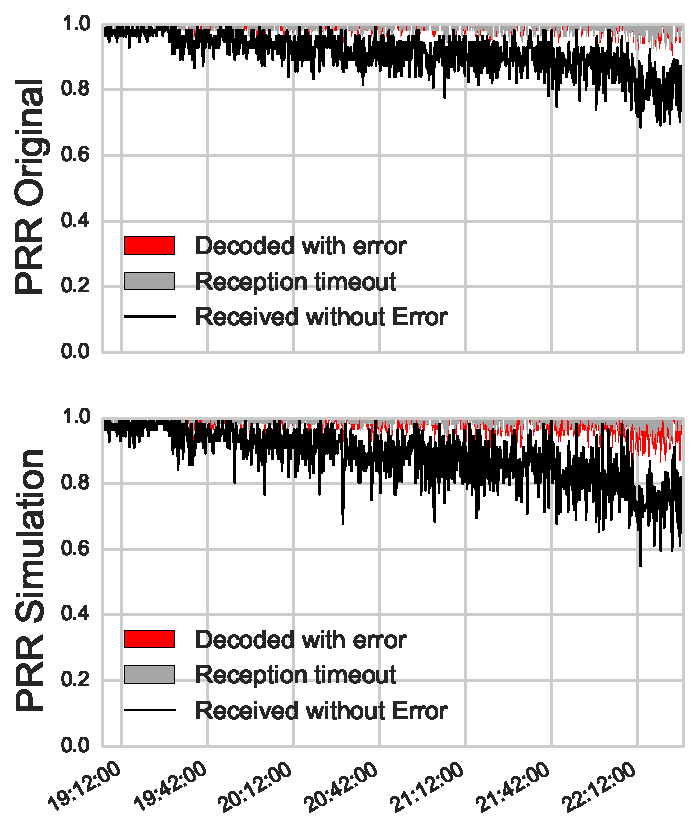
\includegraphics[width=0.475\columnwidth]{figures/fec_scheme_box1_box0_os_1-0_Throughput}
		\label{fig:prr_link_10_transmitter_fec}
	}
	\caption{Original and simulated \acs{PRR} of the two $RS(80,70)$ encoded links of Figure~\ref{fig:prr_link_10}.}
	\label{fig:prr_link_10_fec}
\end{figure}

These results show that this simple simulator is a very good time- and cost-saving alternative to testing the effects of different payloads over a real link, if good original data is available.
Using our trace-based simulator eliminates the effect of uncontrollable environmental factors or hardware issues on repeatability and allows us to focus purely on the message content, without assuming  idealized and monolithic link properties.
